% This LaTeX was auto-generated from MATLAB code.
% To make changes, update the MATLAB code and export to LaTeX again.

\documentclass{article}

\usepackage[utf8]{inputenc}
\usepackage[T1]{fontenc}
\usepackage{lmodern}
\usepackage{graphicx}
\usepackage{color}
\usepackage{hyperref}
\usepackage{amsmath}
\usepackage{amsfonts}
\usepackage{epstopdf}
\usepackage[table]{xcolor}
\usepackage{matlab}

\sloppy
\epstopdfsetup{outdir=./}
\graphicspath{ {./lab1_images/} }

\begin{document}

\matlabtitle{1 - Getting Started}

\begin{par}
\begin{flushleft}
Load the data that we will use.
\end{flushleft}
\end{par}

\begin{matlabcode}
I = imread('lab1/images/napoleon.png');
Il = imread('lab1/images/napoleon_light.png');
Id = imread('lab1/images/napoleon_dark.png');
Z = imread('lab1/images/zebra.png');
\end{matlabcode}


\matlabheading{2 - Viewing Images and Saving Images}

\begin{matlabcode}
imshow(I);
\end{matlabcode}
\begin{center}
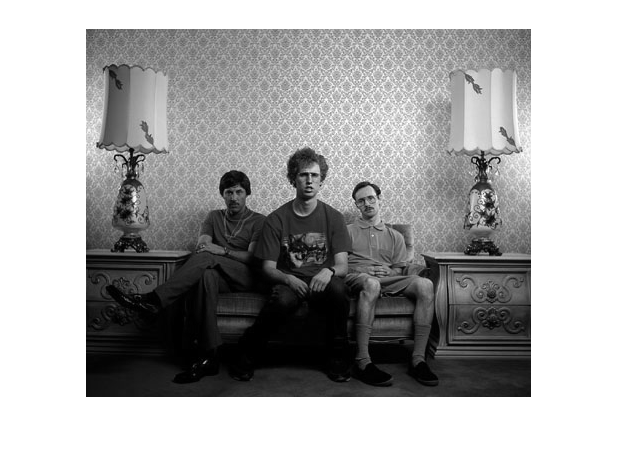
\includegraphics[width=\maxwidth{62.117410938283996em}]{figure_0.png}
\end{center}


\matlabheading{2 - Image Tool}

\begin{matlabcode}
imtool(I);
\end{matlabcode}
\begin{center}
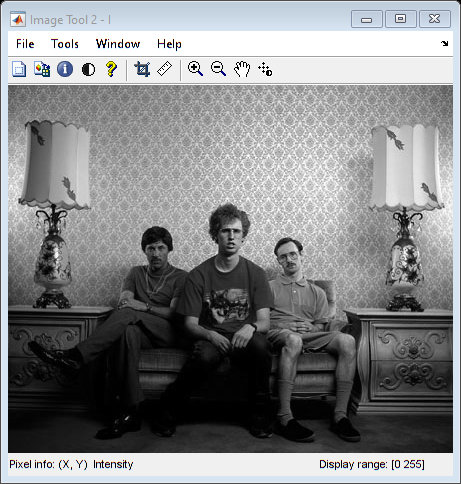
\includegraphics[width=\maxwidth{44.65629703963874em}]{figure_1.png}
\end{center}


\matlabheading{Q1 - Pixel Value}

\begin{par}
\begin{flushleft}
Print out value. We see that it is of type UINT-8 and 
\end{flushleft}
\end{par}

\begin{matlabcode}
I(1, 1)         % It prints out 89
\end{matlabcode}
\begin{matlaboutput}
ans = 89
\end{matlaboutput}


\matlabheading{3 - Contrast, Brightness and Datatypes}

\begin{matlabcode}
imtool(I);
\end{matlabcode}
\begin{center}
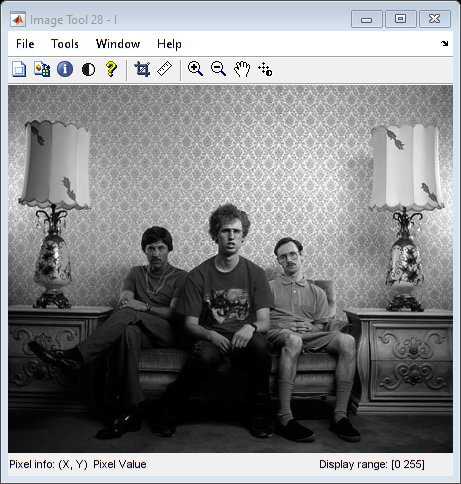
\includegraphics[width=\maxwidth{44.65629703963874em}]{figure_2.png}
\end{center}
\begin{matlabcode}
imtool(Il);
\end{matlabcode}
\begin{center}
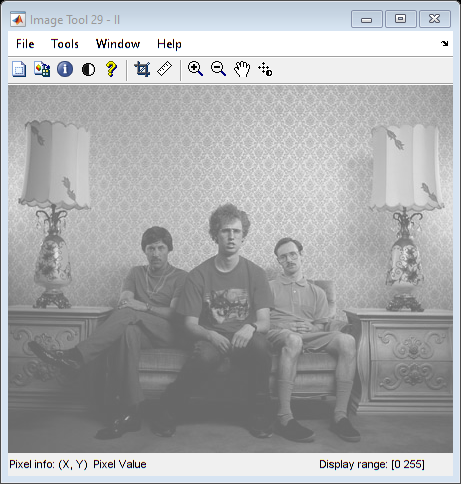
\includegraphics[width=\maxwidth{44.65629703963874em}]{figure_3.png}
\end{center}
\begin{matlabcode}
imtool(Id);
\end{matlabcode}
\begin{center}
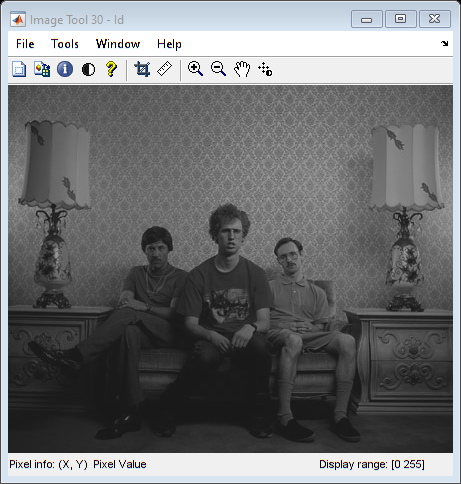
\includegraphics[width=\maxwidth{44.65629703963874em}]{figure_4.png}
\end{center}


\matlabheading{3 Histograms}

\begin{matlabcode}
figure(1);
h1 = histogram(single(I(:)),256);
h1.BinLimits = [0, 255];
grid;
\end{matlabcode}
\begin{center}
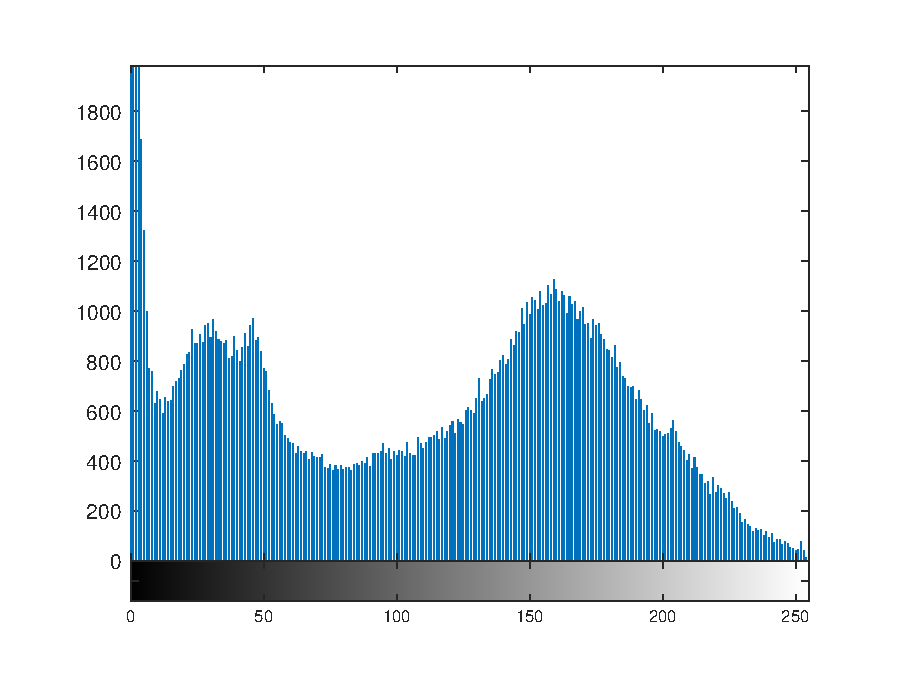
\includegraphics[width=\maxwidth{62.117410938283996em}]{figure_5.eps}
\end{center}
\begin{matlabcode}

figure(2);
h2 = histogram(single(Il(:)),256);
h2.BinLimits = [0, 255];
grid;
\end{matlabcode}
\begin{center}
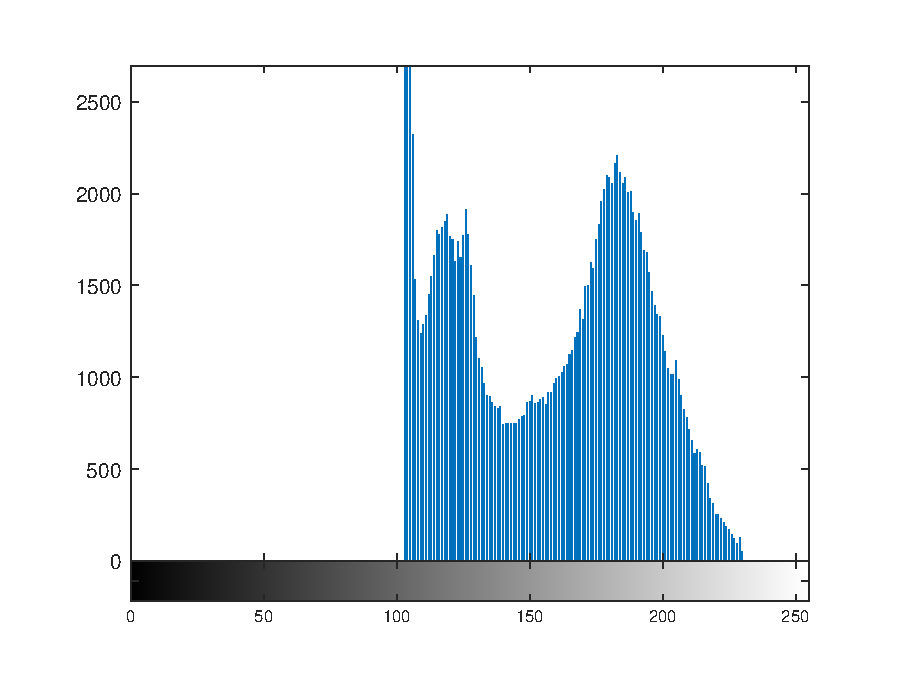
\includegraphics[width=\maxwidth{62.117410938283996em}]{figure_6.eps}
\end{center}
\begin{matlabcode}

figure(3);
h3 = histogram(single(Id(:)),256);
h3.BinLimits = [0, 255];
grid;
\end{matlabcode}
\begin{center}
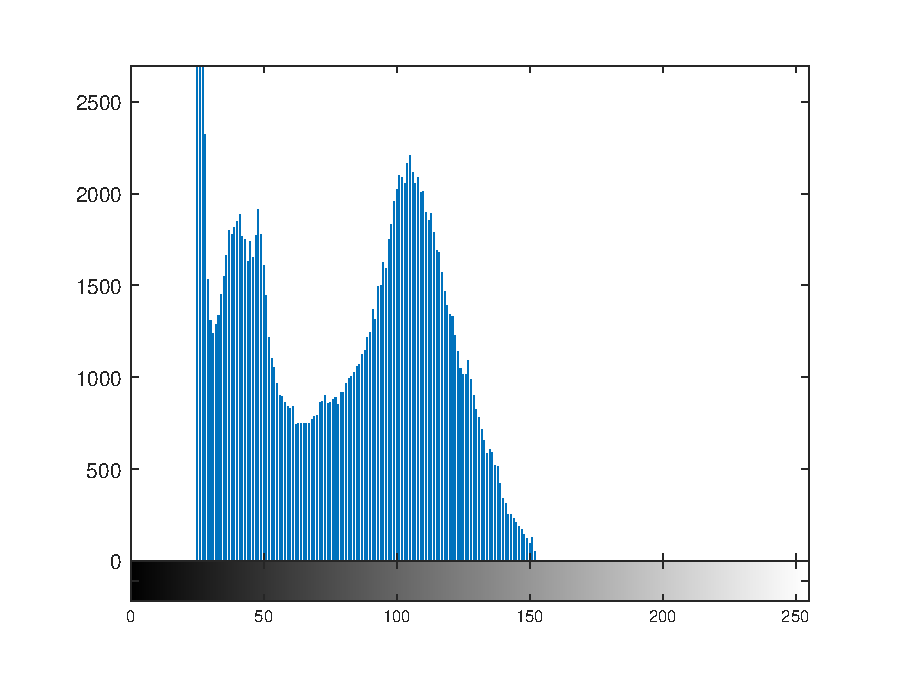
\includegraphics[width=\maxwidth{62.117410938283996em}]{figure_7.eps}
\end{center}


\matlabheading{Explore workspace}

\begin{matlabcode}
whos;
\end{matlabcode}
\begin{matlaboutput}
  Name        Size               Bytes  Class                                        Attributes

  I         368x445             163760  uint8                                                  
  Id        368x445             163760  uint8                                                  
  Il        368x445             163760  uint8                                                  
  Is        368x445             655040  single                                                 
  J         368x445             163760  uint8                                                  
  Jnf        78x78                6084  uint8                                                  
  L         368x445            1310080  double                                                 
  T           1x256               2048  double                                                 
  Z         512x512             262144  logical                                                
  ans         1x1                    1  uint8                                                  
  g           1x1                    8  double                                                 
  h1          1x1                    8  matlab.graphics.chart.primitive.Histogram              
  h2          1x1                    8  matlab.graphics.chart.primitive.Histogram              
  h3          1x1                    8  matlab.graphics.chart.primitive.Histogram              
  out       368x445             163760  uint8                                                  
\end{matlaboutput}
\begin{matlabcode}
class(I);
\end{matlabcode}


\matlabheading{See images}

\begin{matlabcode}
Is = single(I);
imtool(I);
\end{matlabcode}
\begin{center}
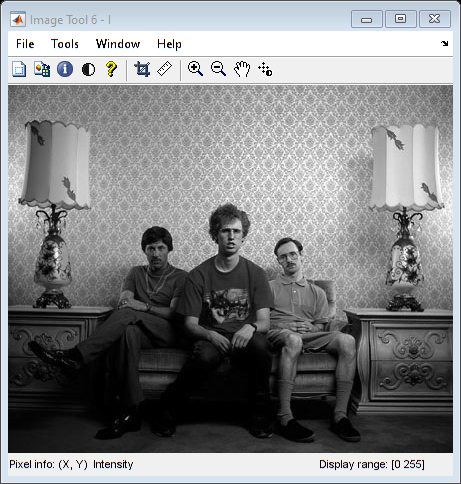
\includegraphics[width=\maxwidth{44.65629703963874em}]{figure_8.png}
\end{center}
\begin{matlabcode}
imtool(Is);
\end{matlabcode}
\begin{center}
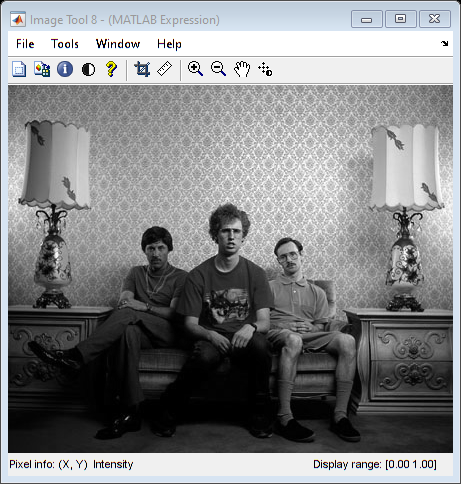
\includegraphics[width=\maxwidth{44.65629703963874em}]{figure_9.png}
\end{center}
\begin{matlabcode}
imtool(Is/255);
\end{matlabcode}
\begin{center}
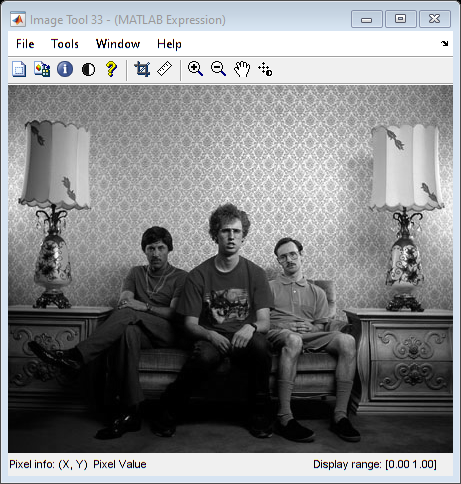
\includegraphics[width=\maxwidth{44.65629703963874em}]{figure_10.png}
\end{center}


\matlabheading{Q3 - Explain differences}

\begin{matlabcode}
figure(1);
imtool((I/64)*64);
\end{matlabcode}
\begin{center}
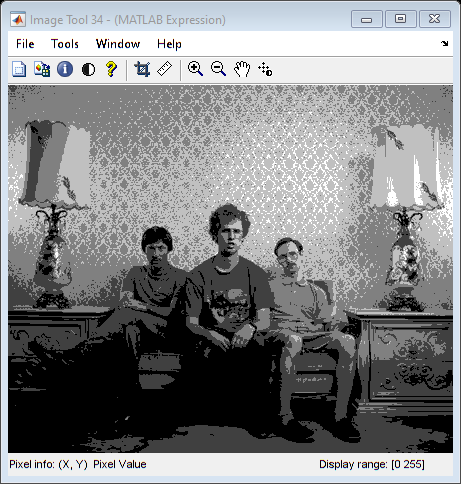
\includegraphics[width=\maxwidth{44.65629703963874em}]{figure_11.png}
\end{center}
\begin{matlabcode}

figure(2);
imtool((Is/64)*64);
\end{matlabcode}
\begin{center}
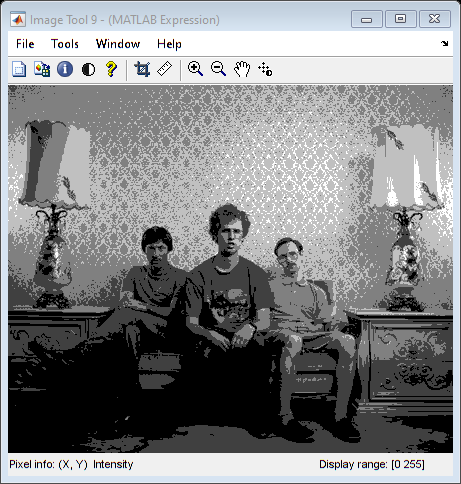
\includegraphics[width=\maxwidth{44.65629703963874em}]{figure_12.png}
\end{center}


\matlabheading{Q4 - Make images brighter}

\begin{matlabcode}
imtool(I + 50);
\end{matlabcode}
\begin{center}
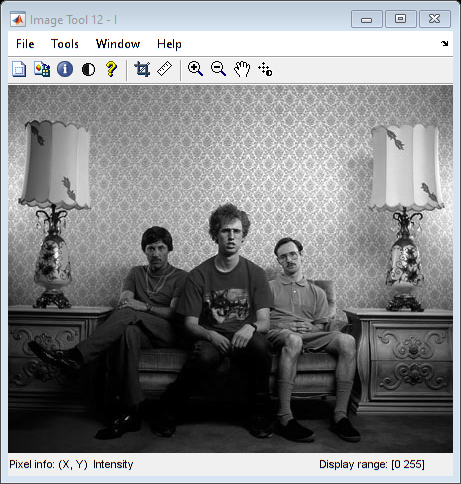
\includegraphics[width=\maxwidth{44.65629703963874em}]{figure_13.png}
\end{center}
\begin{matlabcode}
imtool(I);
\end{matlabcode}
\begin{center}
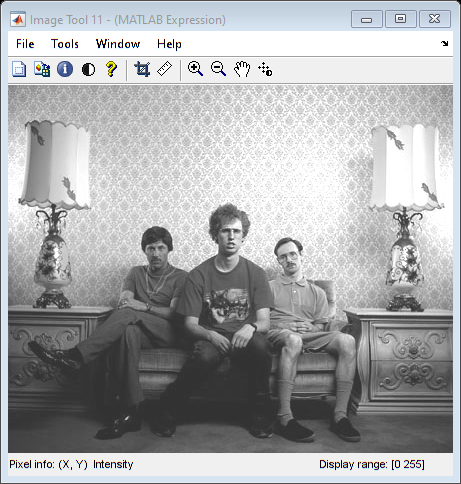
\includegraphics[width=\maxwidth{44.65629703963874em}]{figure_14.png}
\end{center}


\matlabheading{Q5 - Make images lower contrast}

\begin{matlabcode}
imtool(I);
\end{matlabcode}
\begin{center}
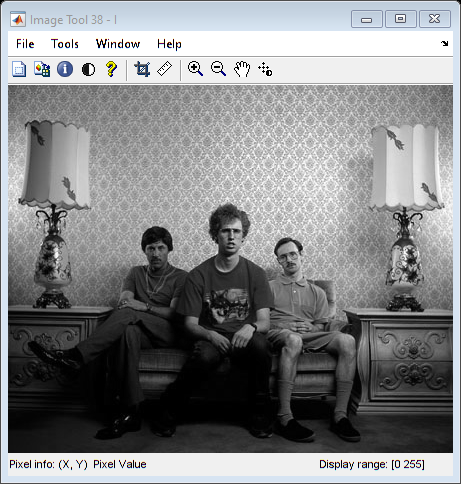
\includegraphics[width=\maxwidth{44.65629703963874em}]{figure_15.png}
\end{center}
\begin{matlabcode}
imtool(I * 0.5);
\end{matlabcode}
\begin{center}
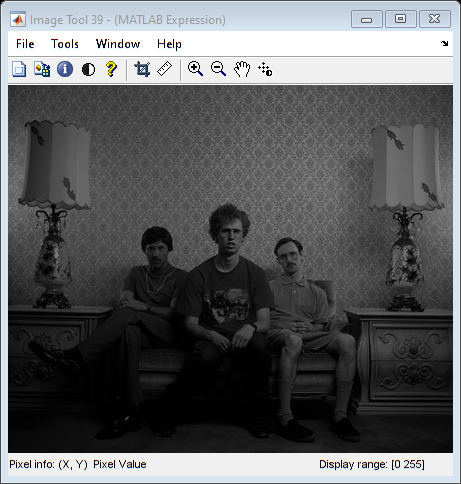
\includegraphics[width=\maxwidth{44.65629703963874em}]{figure_16.png}
\end{center}


\matlabheading{Q6 - Pixel Wise Transforms}

\begin{matlabcode}
figure(1);
imhist(I);
\end{matlabcode}
\begin{center}
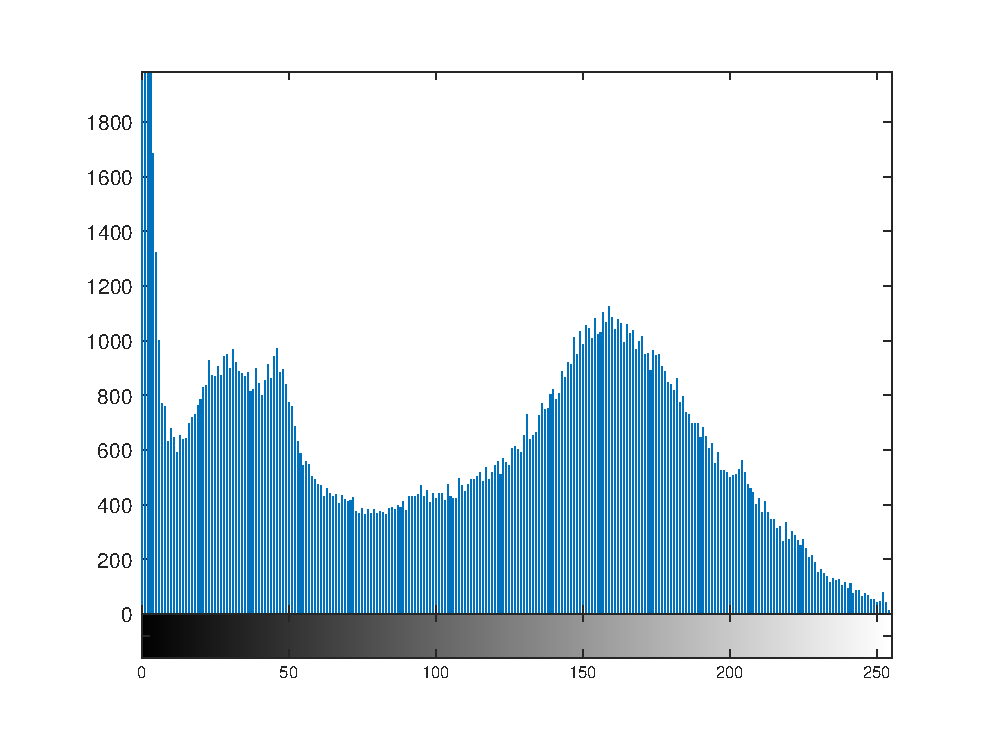
\includegraphics[width=\maxwidth{62.117410938283996em}]{figure_17.eps}
\end{center}
\begin{matlabcode}

figure(2);
imshow(I);
\end{matlabcode}
\begin{center}
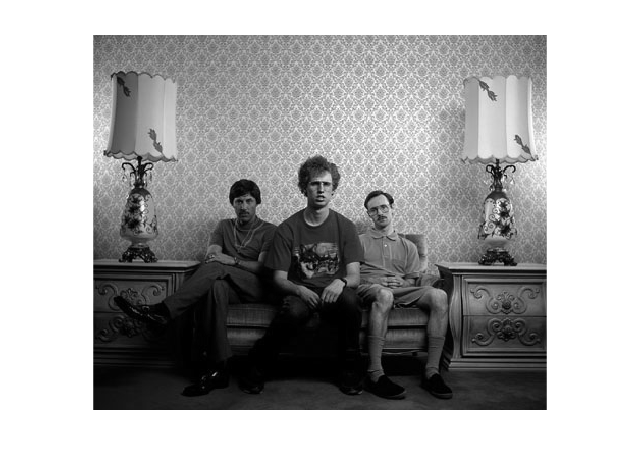
\includegraphics[width=\maxwidth{62.117410938283996em}]{figure_18.png}
\end{center}
\begin{matlabcode}

g = 0.5;
L = double(I).^g;
out = uint8(L .* (255/max(max(L))));

figure(3);
imhist(out);
\end{matlabcode}
\begin{center}
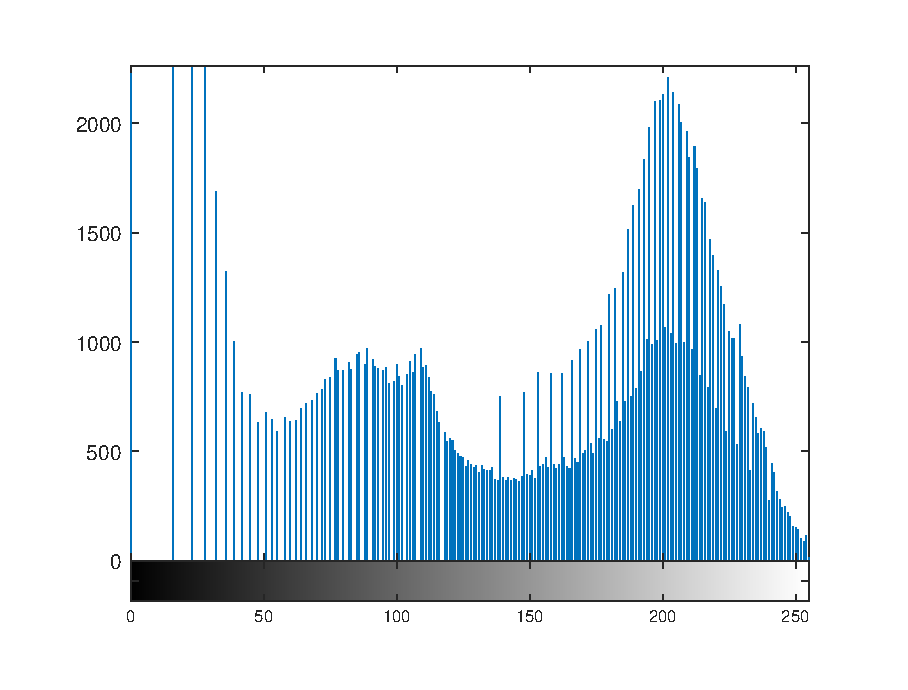
\includegraphics[width=\maxwidth{62.117410938283996em}]{figure_19.eps}
\end{center}
\begin{matlabcode}

figure(4);
imshow(out);
\end{matlabcode}
\begin{center}
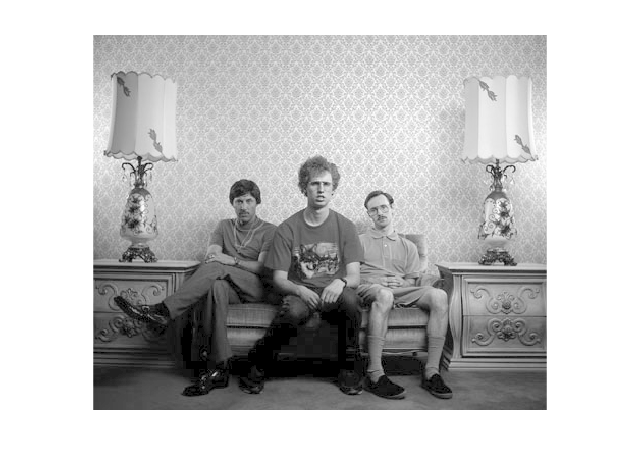
\includegraphics[width=\maxwidth{62.117410938283996em}]{figure_20.png}
\end{center}
\begin{matlabcode}

g = 2;
L = double(I).^g;
out = uint8(L .* (255/max(max(L))));

figure(5)
imhist(out);
\end{matlabcode}
\begin{center}
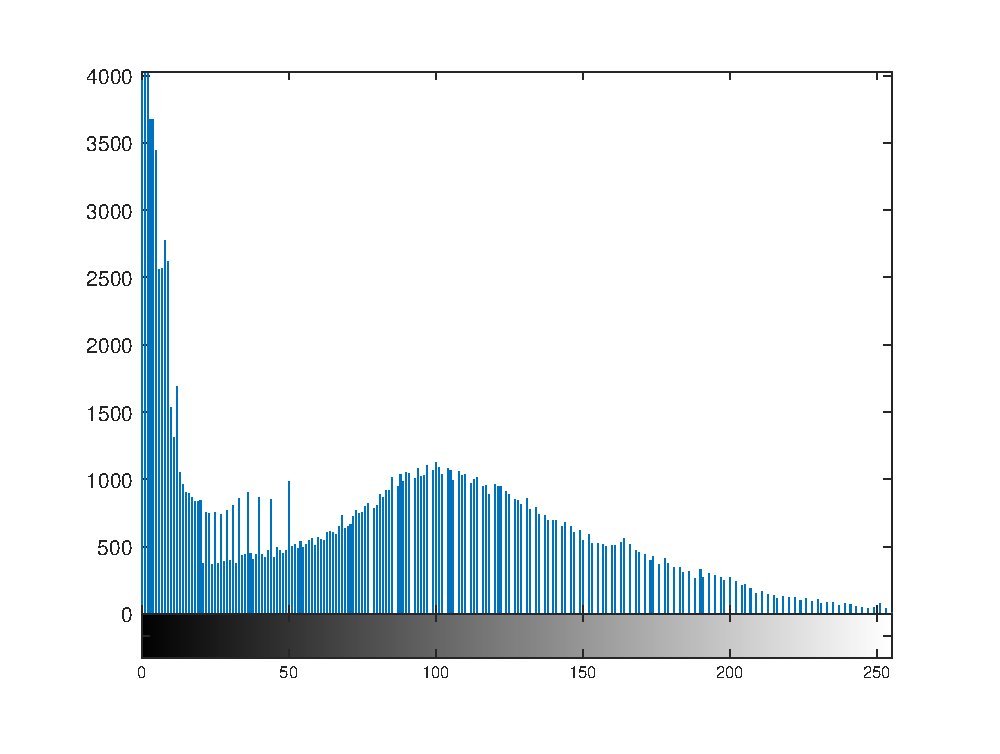
\includegraphics[width=\maxwidth{62.117410938283996em}]{figure_21.eps}
\end{center}
\begin{matlabcode}

figure(6);
imshow(out);
\end{matlabcode}
\begin{center}
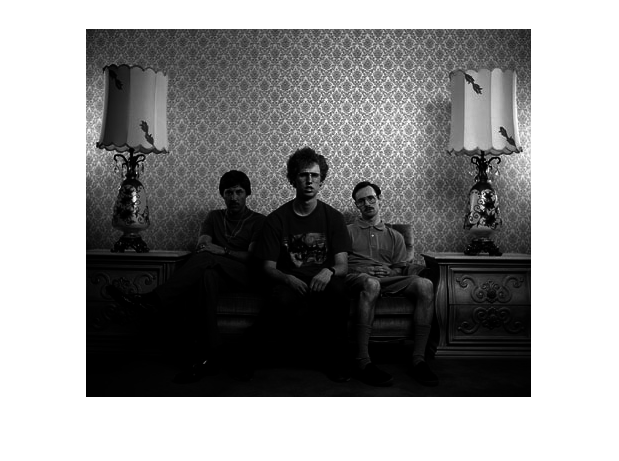
\includegraphics[width=\maxwidth{62.117410938283996em}]{figure_22.png}
\end{center}


\matlabheading{Q7 - Histogram Equalization napoleon - Histogram}

\begin{matlabcode}
figure(1);
imhist(I);
\end{matlabcode}
\begin{center}
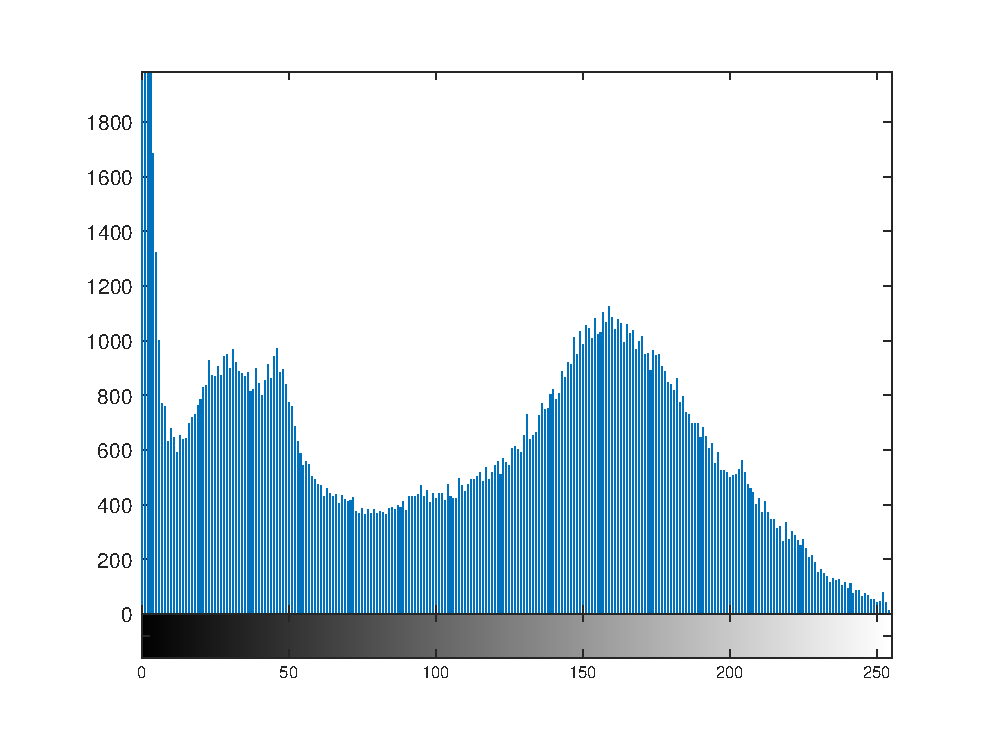
\includegraphics[width=\maxwidth{62.117410938283996em}]{figure_23.eps}
\end{center}
\begin{matlabcode}

figure(2);
imhist(histeq(I));
\end{matlabcode}
\begin{center}
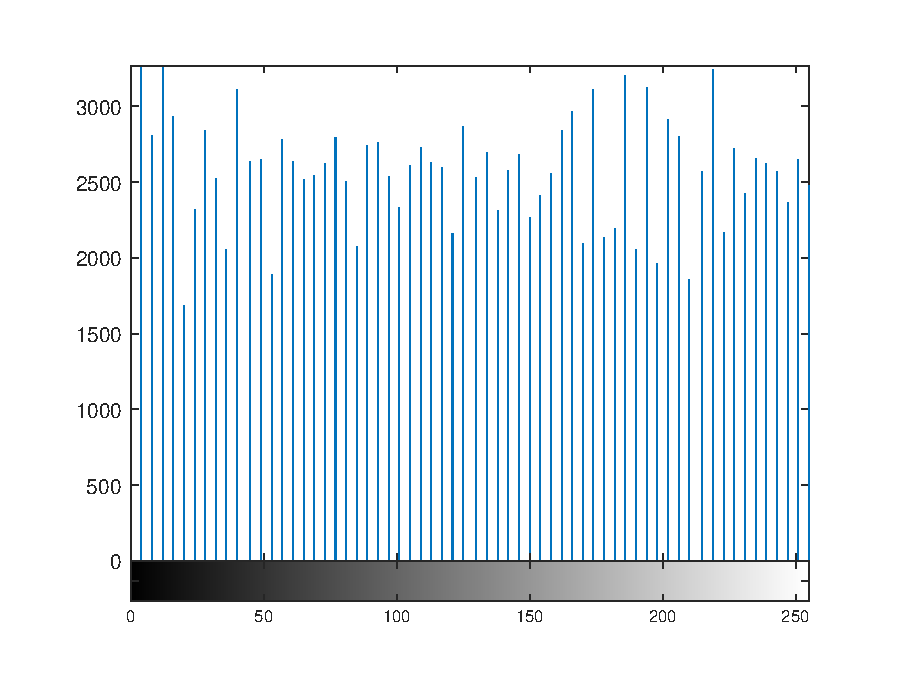
\includegraphics[width=\maxwidth{62.117410938283996em}]{figure_24.eps}
\end{center}
\begin{matlabcode}

figure(3);
imhist(histeq(Il));
\end{matlabcode}
\begin{center}
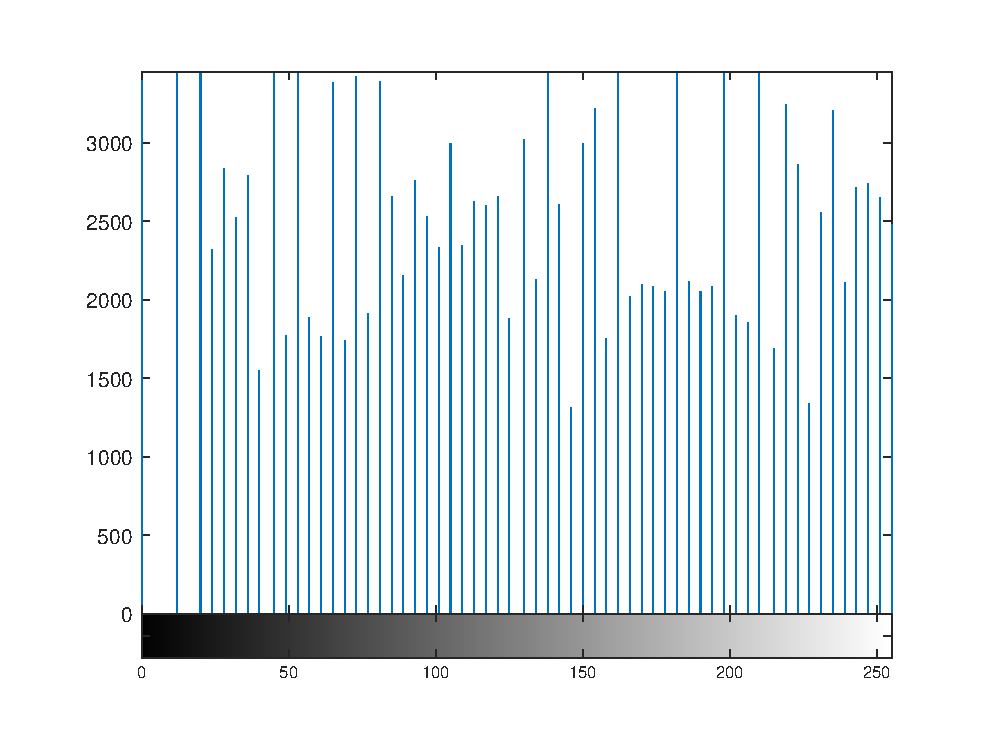
\includegraphics[width=\maxwidth{62.117410938283996em}]{figure_25.eps}
\end{center}
\begin{matlabcode}

figure(4);
imhist(histeq(Id));
\end{matlabcode}
\begin{center}
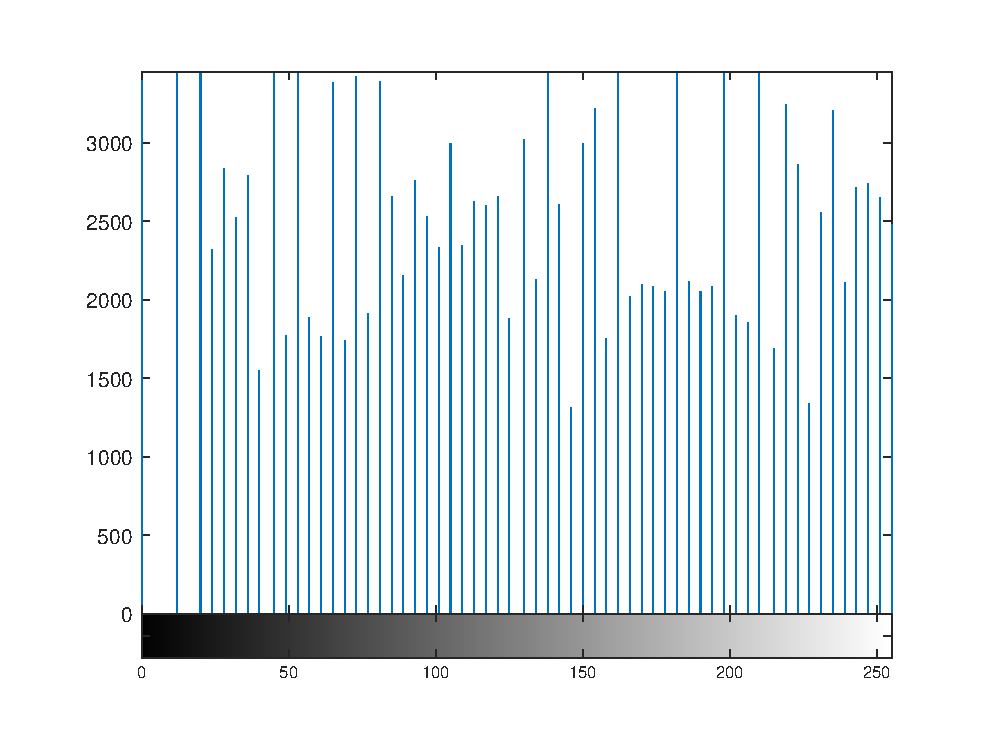
\includegraphics[width=\maxwidth{62.117410938283996em}]{figure_26.eps}
\end{center}


\matlabheading{Q7 - Histogram Equalization napoleon - Images}

\begin{matlabcode}
figure(1);
imshow(I);
\end{matlabcode}
\begin{center}
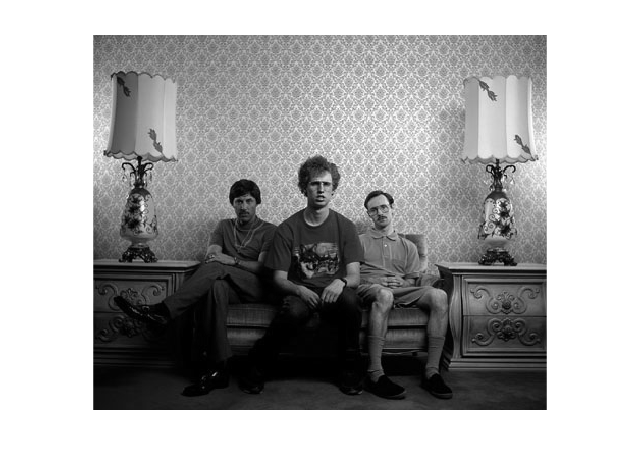
\includegraphics[width=\maxwidth{62.117410938283996em}]{figure_27.png}
\end{center}
\begin{matlabcode}

figure(2);
imshow(histeq(I));
\end{matlabcode}
\begin{center}
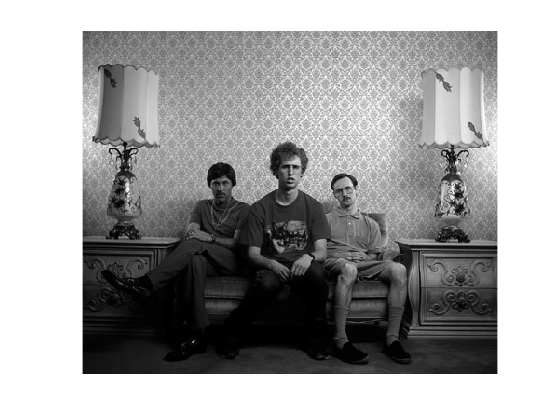
\includegraphics[width=\maxwidth{62.117410938283996em}]{figure_28.png}
\end{center}
\begin{matlabcode}

figure(3);
imshow(histeq(Il));
\end{matlabcode}
\begin{center}
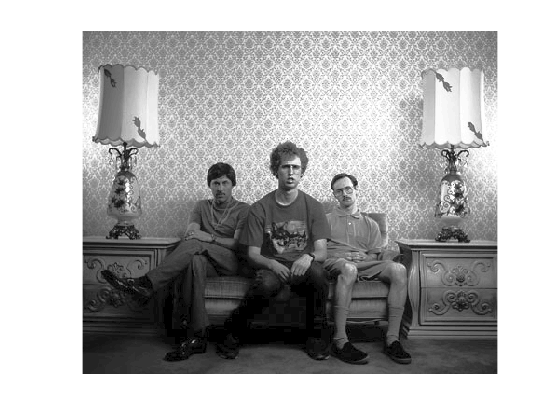
\includegraphics[width=\maxwidth{62.117410938283996em}]{figure_29.png}
\end{center}
\begin{matlabcode}

figure(4);
imshow(histeq(Id));
\end{matlabcode}
\begin{center}
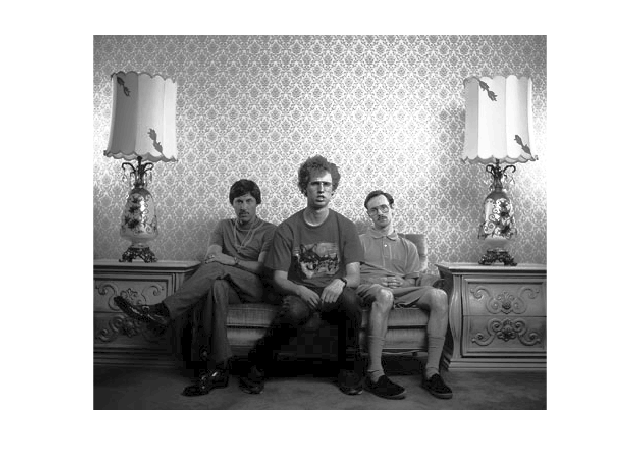
\includegraphics[width=\maxwidth{62.117410938283996em}]{figure_30.png}
\end{center}


\matlabheading{Q7 - Histogram, transform and cumulative histogram - Regular Image}

\begin{matlabcode}
[J,T] = histeq(I);

figure
plot((0:255)/255,T);
\end{matlabcode}
\begin{center}
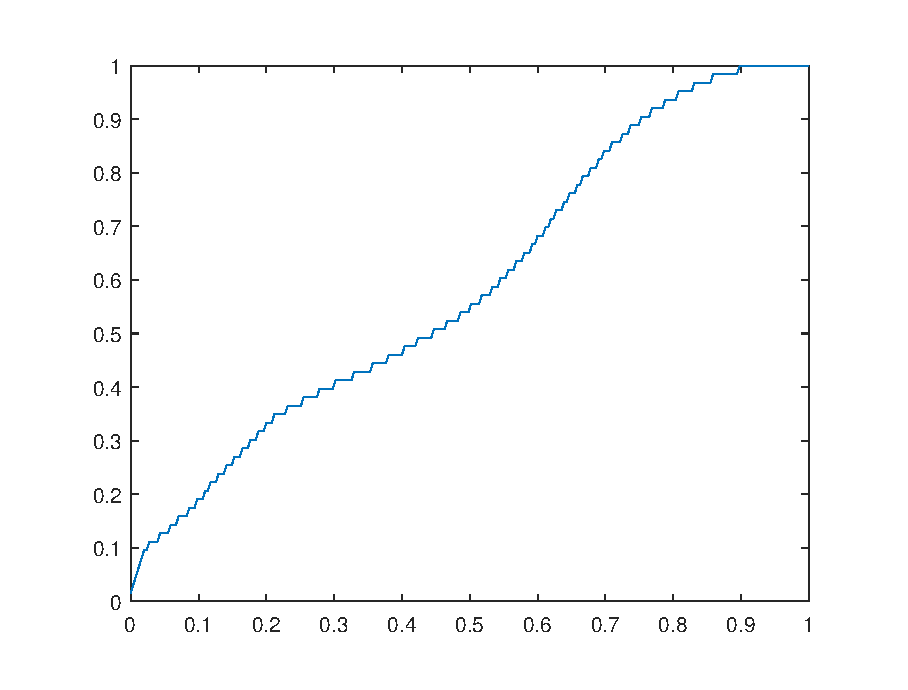
\includegraphics[width=\maxwidth{56.196688409433015em}]{figure_31.eps}
\end{center}
\begin{matlabcode}

figure
plot(cumsum(imhist(I)) / sum(imhist(I)));
\end{matlabcode}
\begin{center}
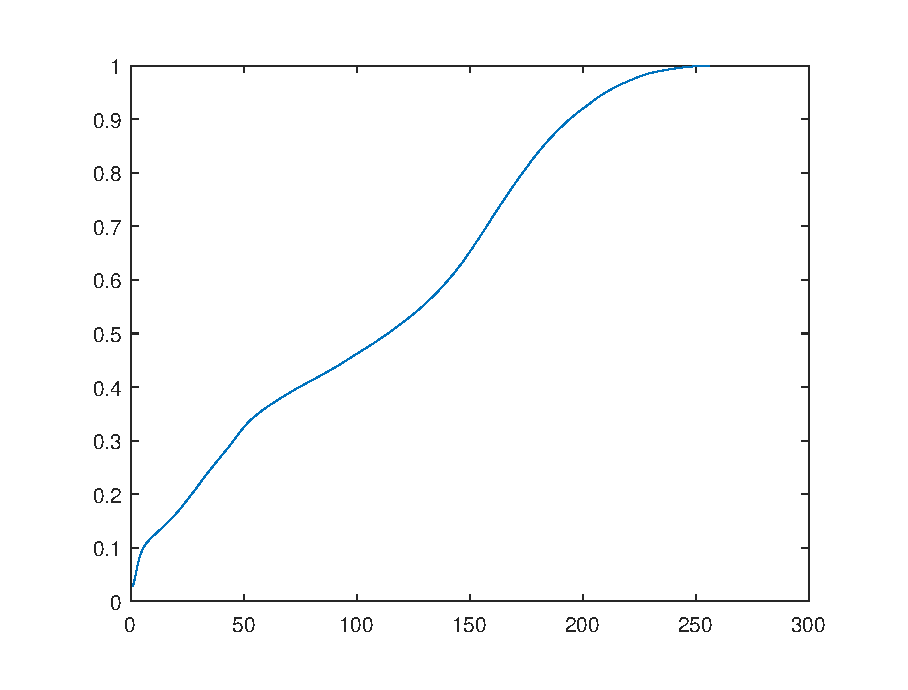
\includegraphics[width=\maxwidth{56.196688409433015em}]{figure_32.eps}
\end{center}
\begin{matlabcode}

figure
plot(cumsum(imhist(J)) / sum(imhist(J)));
\end{matlabcode}
\begin{center}
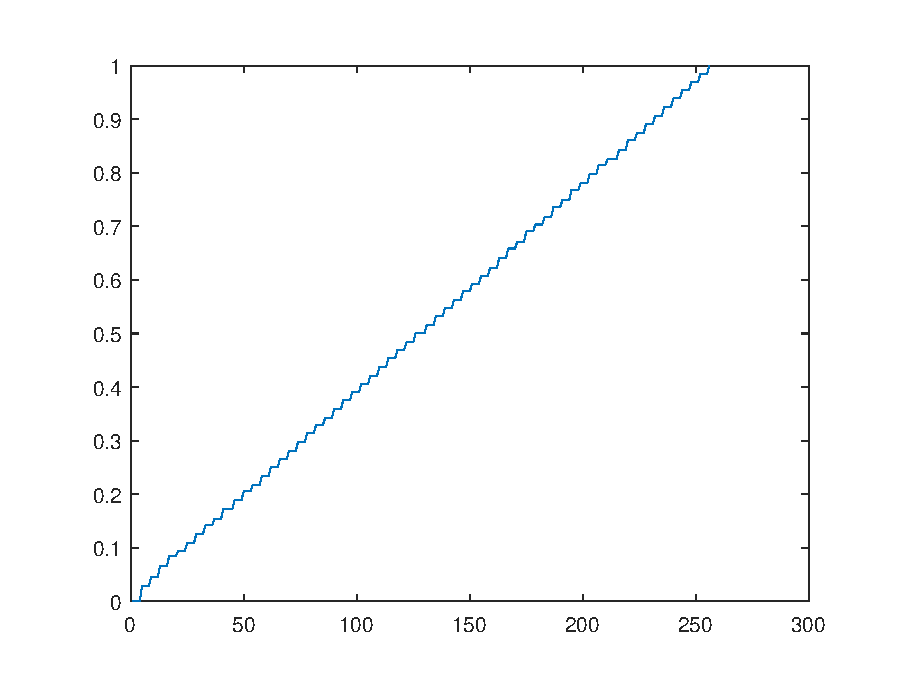
\includegraphics[width=\maxwidth{56.196688409433015em}]{figure_33.eps}
\end{center}


\matlabheading{Q7 - Histogram, transform and cumulative histogram - Light}

\begin{matlabcode}
[J,T] = histeq(Il);

figure
plot((0:255)/255,T);
\end{matlabcode}
\begin{center}
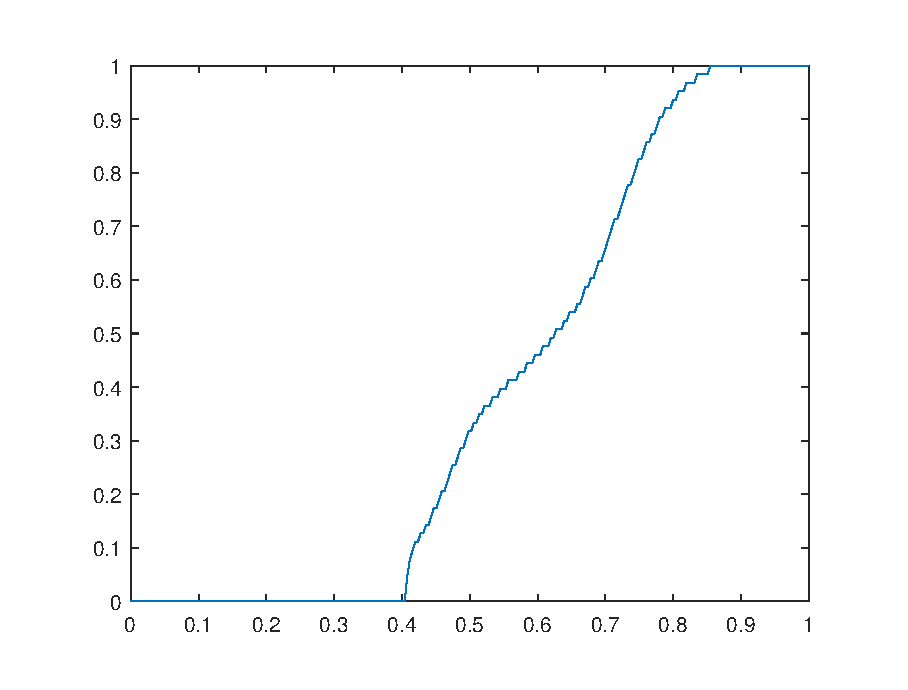
\includegraphics[width=\maxwidth{56.196688409433015em}]{figure_34.eps}
\end{center}
\begin{matlabcode}

figure
plot(cumsum(imhist(Il)) / sum(imhist(Il)));
\end{matlabcode}
\begin{center}
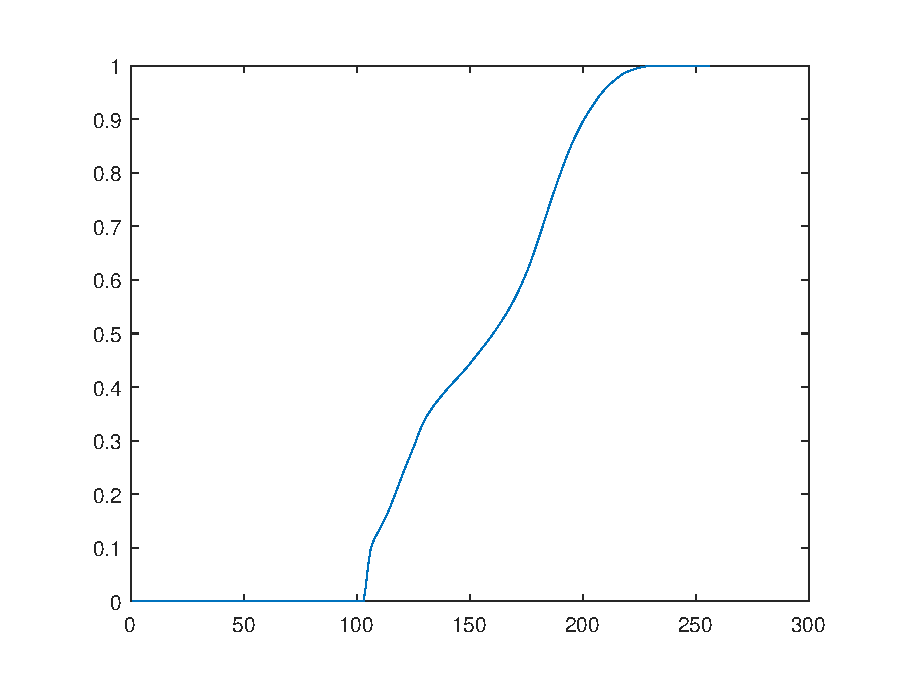
\includegraphics[width=\maxwidth{56.196688409433015em}]{figure_35.eps}
\end{center}
\begin{matlabcode}

figure
plot(cumsum(imhist(J)) / sum(imhist(J)));
\end{matlabcode}
\begin{center}
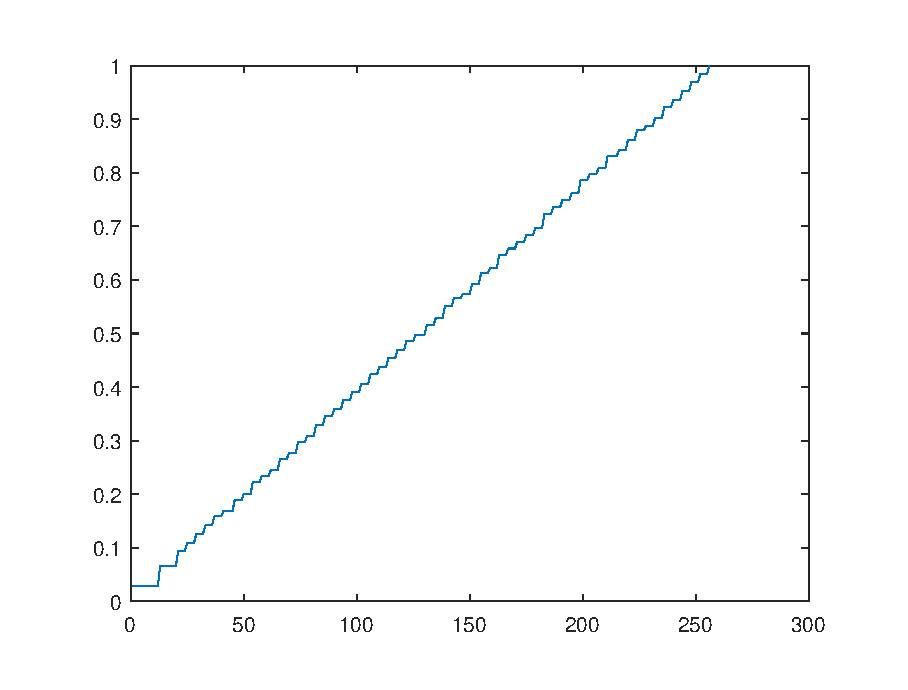
\includegraphics[width=\maxwidth{56.196688409433015em}]{figure_36.eps}
\end{center}


\matlabheading{Q7 - Histogram, transform and cumulative histogram - Dark}

\begin{matlabcode}
[J,T] = histeq(Id);

figure
plot((0:255)/255,T);
\end{matlabcode}
\begin{center}
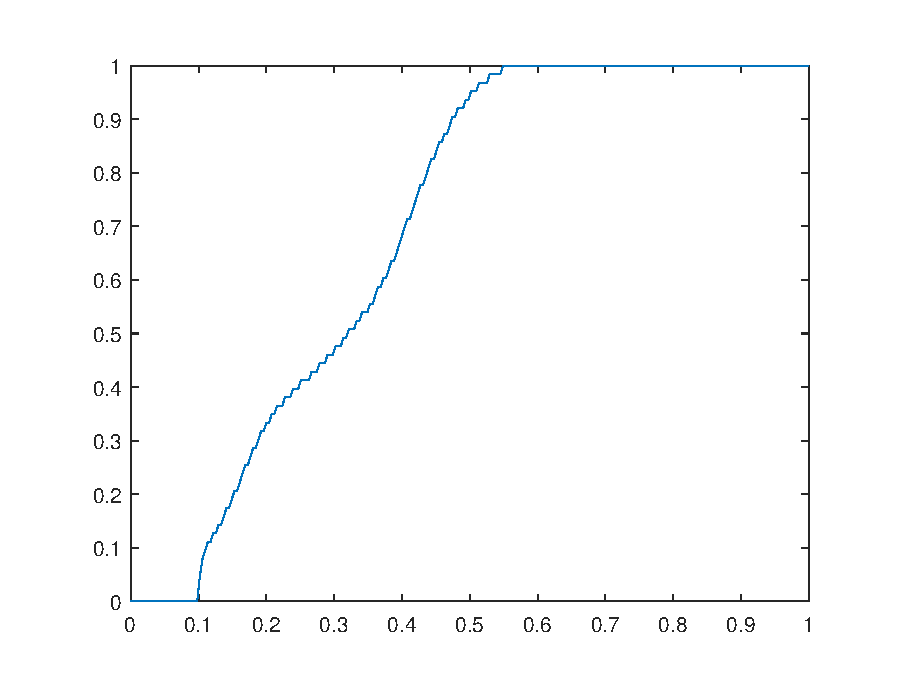
\includegraphics[width=\maxwidth{56.196688409433015em}]{figure_37.eps}
\end{center}
\begin{matlabcode}

figure
plot(cumsum(imhist(Id)) / sum(imhist(Id)));
\end{matlabcode}
\begin{center}
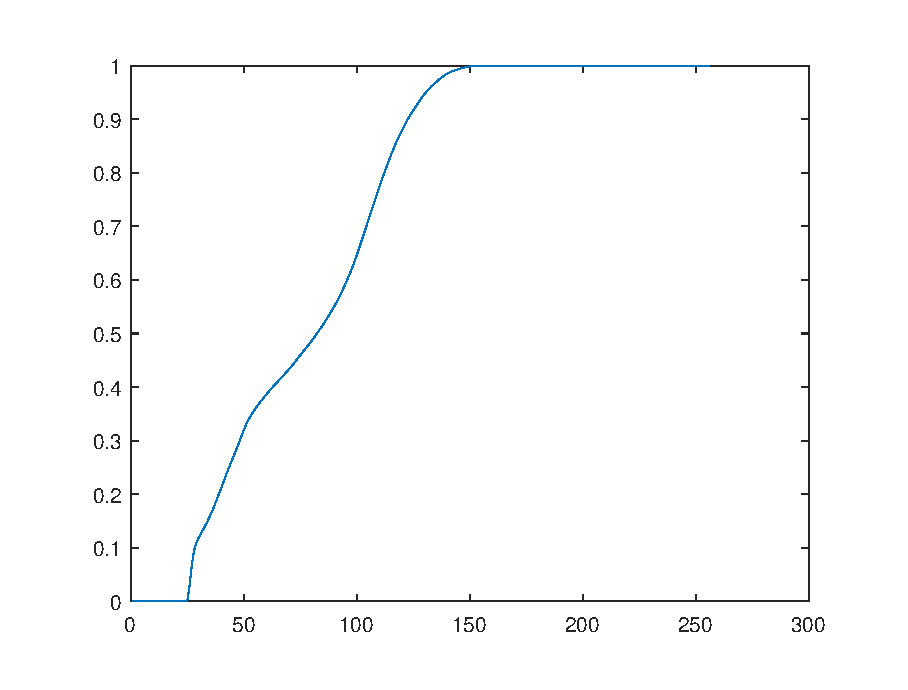
\includegraphics[width=\maxwidth{56.196688409433015em}]{figure_38.eps}
\end{center}
\begin{matlabcode}

figure
plot(cumsum(imhist(J)) / sum(imhist(J)));
\end{matlabcode}
\begin{center}
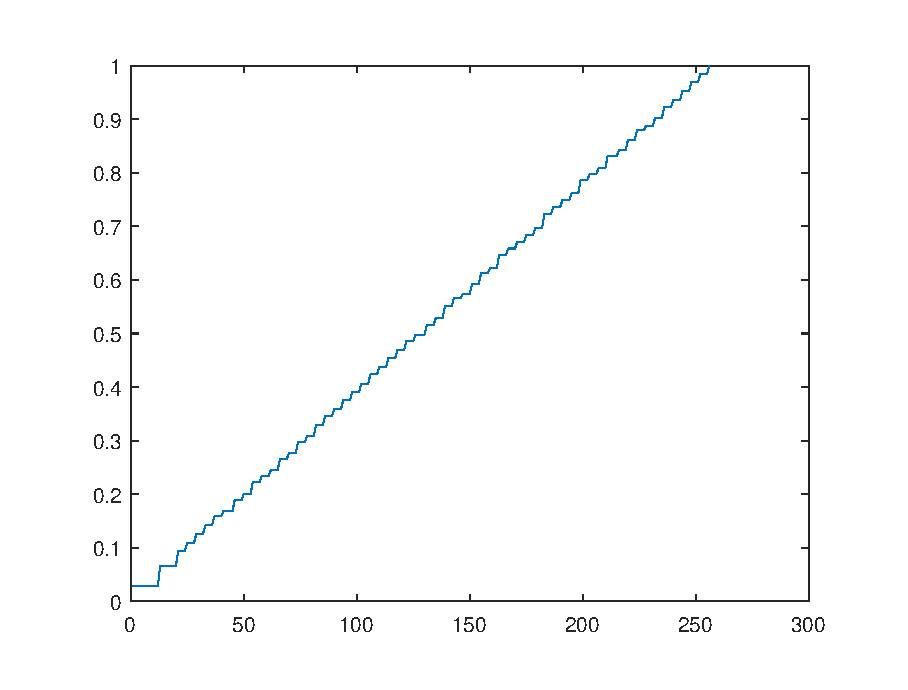
\includegraphics[width=\maxwidth{56.196688409433015em}]{figure_39.eps}
\end{center}


\matlabheading{Q8 - Aliasing when sampling}

\begin{matlabcode}
Jnf = imresize(I, [78 78], 'nearest', 'antialiasing', false);
imshow(Jnf);
\end{matlabcode}
\begin{center}
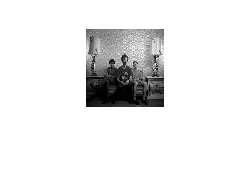
\includegraphics[width=\maxwidth{25.28850978424486em}]{figure_40.png}
\end{center}

\end{document}
